%% The first command in your LaTeX source must be the \documentclass command.
%%
%% Options:
%% twocolumn : Two column layout.
%% hf: enable header and footer.
\documentclass[
 twocolumn,
 hf,
]{ceurart}

%%
%% One can fix some overfulls
\sloppy

%%
%% Minted listings support 
%% Need pygment <http://pygments.org/> <http://pypi.python.org/pypi/Pygments>
\usepackage{lmodern}
\usepackage{textcomp}
\usepackage{listings}
\usepackage{minted}

%% auto break lines
\lstset{breaklines=true}

%%
%% end of the preamble, start of the body of the document source.
\begin{document}

%%
%% The "title" command
\title{Explain your clusters with words. The role of metadata in interactive clustering}

%%
%% The "author" command and its associated commands are used to define
%% the authors and their affiliations.
\author[1]{Maciej Mozolewski}[
  orcid=0000-0003-4227-3894,
  email=m.mozolewski@doctoral.uj.edu.pl,
  url=https://github.com/mozo64,
]

\author[2]{Samaneh Jamshidi}[
  orcid=0000-0001-7055-2706,
  email=samaneh.jamshidi@hh.se,
]

\author[1]{Szymon Bobek}[
  orcid=0000-0002-6350-8405,
  email=szymon.bobek@uj.edu.pl,
]

\author[1]{Grzegorz J. Nalepa}[
  orcid=0000-0002-8182-4225,
  email=grzegorz.j.nalepa@uj.edu.pl,
]

\address[1]{Jagiellonian Human-Centered Artificial Intelligence Laboratory (JAHCAI) and Institute of Applied Computer Science, Jagiellonian University, Cracow, Poland}
\address[2]{Center for Applied Intelligent Systems Research (CAISR), Halmstad University, Halmstad, Sweden}

%%
%% Rights management information.
%% CC-BY is default license.
\copyrightyear{2022}
\copyrightclause{Copyright for this paper by its authors.
Use permitted under Creative Commons License Attribution 4.0
International (CC BY 4.0).}

%%
%% This command is for the conference information
\conference{IJCAI-ECAI 2022, the 31st International Joint Conference on Artificial Intelligence and the 25th European Conference on Artificial Intelligence, July 23--29, 2022
Messe Wien, Vienna, Austria}

%\maketitle

%%
%% The abstract is a short summary of the work to be presented in the
%% article.
\begin{abstract}
  In this preliminary work, we present an approach for augmentation of clustering with natural language explanations.
  In clustering there are 2 main challenges: a) choice of a proper, reasonable number of clusters and b) cluster analysis and profiling.
  There is a plethora of technics for a) but not so much for b), which is in general a laborious task of explaining obtained clusters.
  %Clustering is in a sense art in that regard that it is an intuitive and iterative process. % This sentence is strange...
  %Therefore, XAI techniques are well suited in this area.
  In this work, we propose a method that aids experts in cluster analysis by providing iterative, human-in-the-loop methodology of generating cluster explanations.
  In a convincing example, we show how the process of clustering on a set of \textit{objective variables} could be facilitated with textual \textit{metadata}.
  In our case, images of products from online fashion store are used for clustering.
  Then, product descriptions are used for profiling clusters.
\end{abstract}

%%
%% Keywords. The author(s) should pick words that accurately describe
%% the work being presented. Separate the keywords with commas.
\begin{keywords}
  XAI \sep
  clustering \sep
  metadata \sep
  Natural Language Processing \sep
  explanations \sep
  narratives
\end{keywords}

%%
%% This command processes the author and affiliation and title
%% information and builds the first part of the formatted document.
\maketitle

\section{Introduction}\label{sec:introduction}
%In general what is the prroblem -- in clustering we need to analyse results, XAI can help us in doing that
%- classification as a tool for understanding
Data analysts and data scientists are often faced with the task of describing phenomena in a way that is understandable to the audience.
On the one hand, they have some data that they can describe statistically, categorize, or predict events based on it, etc.
On the other hand, they want to deliver their observations in some kind of narrative that they can "sell" to decision-makers.
There is even a phenomenon called \textit{data storytelling}.
In our work we want to show that this intuitive approach is reflected in the work of these people, which manifests itself in the way they use different types of data.

Assigning labels to groups of similar objects is one of the ways how humans describe the world~\cite{Rosch1978-ROSCAC-5}.
It begins with the notion that some phenomena or entities differ from each other and that they could be divided into distinct classes.
Clarification of the differences between groups gets better and better along with the knowledge gained about the instances that form different groups.
Finally, one is giving names to those different categories of entities. %TODO: can we cite some work from social sicence whcih actually is about that?
In essence, clustering in machine learning is no different process.

%- the problem is common in fields like: marketing, e-commerce, industries, ???
%- one like to classify \textit{objective data} like images, sensors, etc to uncover hidden structure
%- to many observations to do it manually
%Clustering methods are standard in many fields of human prosperity.
%In the advent of an ever-increasing amount of data, we use tools to automate the process, as manual clustering is too laborious.
%Indeed, there are many statistical, machine learning, and deep learning algorithms.
%The difficulty arises to convince end-users that derived clusters make sense.
%Will it be clustering sensor data in Industry 4.0 or behaviors of consumers, results need to be actionable.
%We believe that this is impossible if we do not explain what the algorithm has learned. % and if it is of any value for humans.
%We continually hypothesize about the significant differences between classes, then test results
Clustering is an intrinsically subjective task and requires human assessment~\cite{10.1145/3340960}.
It is a purely statistical method which finds homogeneous groups of entities.
It belongs to the family of unsupervised learning algorithms in contrast to classification or regression, which are supervised.
At every step of this process, the user makes decisions based on her/his domain knowledge.
First, the user needs to select features (variables) used by the algorithm.
Secondly, the user selects the type of algorithm, similarity measures, number of clusters or size of the smallest one.
Finally, she or he checks clusters by describing objects belonging to subsequent groups.
It also follows that the process is iterative.

%- explanations needs to be done with data comprehensible by humans
%   - data are not equal
%  - images are self-explanatory in e-commerce setting, but not necessarily in other (vide images of medical images, satellites,  etc)
%  - industrial data - rarely
%  - thus "metadata" - link between "objective/hard" data and "soft" - like labels given by humans eg descriptions of products
%  - higher probability of bias
%  - sanity check of metadata
From our expertise in e-commerce and Industry 4.0, we often see distinctions between two types of data.
There are \textit{objective data} and the \textit{subjective data} or \textit{metadata}.
For instance, in e-commerce popular approach for recommendations is based on finding users similar to each other in terms of interactions with products.
Thus, \textit{objective data} is composed of the behaviors of shoppers.
The categories, titles and descriptions of the products form \textit{metadata}, which is usually the result of the joint work of many employees of the e-store.
For rolling steel factories, predictive maintenance models are derived mainly from \textit{objective sensory data}, such as temperature, force, etc.
Factory accounting data are \textit{metadata}.
%Six-sigma quality standards lay somewhere in between of \textit{objective-subjective} continuum.
Going back to narratives, \textit{objective data} can be viewed as story or the totality of facts that have occurred.
They can be difficult for humans to understand but lend themselves well to clustering.
\textit{Metadata}, in contrast, is more a type of narrative, or how the algorithm's outcome is presented by data scientists to their audience.
\textit{Metadata} is more subjective, making it more suitable for justification and formulation of conclusions and explanations.

%Our underlying statement is.
%This leads to the conclusion:
The more \textit{objective} the data is, the more it is suited for modeling the phenomena, be it physical, business, sociological or psychological in nature.
\textit{Metadata} is more suitable for explaining the model to the user, convincing her or him, and prompting to make decisions and actions based on this knowledge.
It is more prone to error because of its conventionality and subjectivity, but they speak to humans.
%- one want to have influence on final outcome
%  - as it is exploratory, it is unsupervised
%  - no direct influence -> to adress this ...
%As a closing remark in this section, we want to pinpoint that humans seek agency.
%Clustering algorithms are unsupervised.
%XAI methods are well-fitted for the job of giving control, both in the clustering stage and profiling stage.

In this work we propose a method that allows for clustering dataset with \textit{objective data}, and explain differences between clusters with \textit{metadata}.
We use XAI methods to explain differences between clusters using \textit{metadata} which is perfectly understandable by humans, but may not be of sufficient quality to perform valid clustering.
The selection of the most interpretable \textit{metadata} is iterative and human-guided.
In our example, we show how image-based clustering can be enhanced with textual description of clusters.
We argue that such an approach can lead to better utilisation of \textit{metadata} for cluster analysis purposes, which results in better understanding of clusters which is the final goal of every clustering task. % BETTER means nothing, but lets keep it that way.
Furthermore, it allows for checking the consistency between two or more possible instance representations (image and text) which might be crucial in domains that rely on both (e.g.\ e-commerce).

The rest of the paper is organized as follows.
In Section~\ref{sec:sota} we present current research in the area of interactive clustering and human-guided cluster analysis.
The description of our method along with use-case studies is given in Section~\ref{sec:clumeta}.
Finally, we conclude our work and show perspectives of its further development is presented in Section~\ref{sec:summary}.

\section{Related works}
\label{sec:sota}
%How this is done in the field
%TODO Parisa

In the survey on interactive clustering~\cite{10.1145/3340960} authors have distinguished 2 groups of approaches in terms of how interaction occurs.
In general, users can interact indirectly with the tool, by changing the parameters of the algorithm, or directly by giving feedback to the result of clustering.
The parameters adjusted most frequently are the number of clusters and the similarity threshold~\cite{10.1007/978-3-319-23461-8_43,10.1016/j.eswa.2017.11.055}.
For topic modeling, users are given the option to select keywords and set their relative importance~\cite{ElAssady2018ProgressiveLO}. %,Choo2013UTOPIANUT}.
On the other hand, direct feedback might be realized by highlighting incorrect instances of splitting or merging the resulting clusters~\cite{10.1155/2017/4915828}. %,10.1111/j.1467-8659.2012.03108.x}.
For textual data, users can provide the tool with blacklists of incorrect topic labels or set similar restrictions~\cite{Chang2016AppGrouperKI}. %,hu-etal-2011-interactive}.
Based on this signal, the clustering tool learns user preferences and tries to incorporate the knowledge in the next iteration.

Explainable AI approaches have become particularly important, and although most work is generally focused on supervised learning, some works have been done to explain clusters.
One of the most common methods for understanding clustering methods is visualization. 
By using low-dimensionality embedding and displaying them in two- or three-dimensional dimensions, one can get an overview of the clusters and their data. 
However, these visualizations are not always understandable and explainable. 

The decision tree is one of the inherently interpretable algorithms. 
So one common way to explain models is to use decision trees. 
Nevertheless, the critical point for explaining the decision tree is its depth because decision trees with high depth no longer are interpreted, so we must pay attention to the depth of the tree produced. 
Using a small decision tree to divide a dataset into k clusters provides explainable clusters, but this approach has a trade-off between being explainable and accuracy. 
IMM algorithm~\cite{dasgupta2020explainable} approximates k-means and k-median clustering by a threshold tree with k leaves.
ExKMC~\cite{frost2020exkmc} uses a threshold tree to provide an explainable k-mean clustering in which the number of tree leaves is greater than the number of clusters.

Besides, visualization or providing some conditions on features, using text data is reasonable to generate explanations to users.
In~\cite{hendricks2016generating} authors use captions of the images along with the images to create a more discriminative classification. 
In addition, they use this \textit{metadata} to provide language explanation and generate a text description for each class.
However, by blending textual and image modalities into one datset, authors limit the possibility of checking consistency between these two types of data and implicitly assume the correctness of possibly wrong image descriptions.

Similarly, in many other methods that aim at explaining differences between discovered clusters, the clustering task is transformed to classification one, and the classifier is then explained with available XAI methods such as LIME~\cite{lime}, Anchor~\cite{anchor}, LUX~\cite{lux2021iccs}, etc.
One of the most recent implementations of such approach can be found in~\cite{xaiclust2021}.

Another approach is given in~\cite{knac2021arxiv}, where authors present a toolkit for conformance checking between expert knowledge and automatic clustering.
The differences between expert-based clustering and automated clustering are justified with XAI methods and the process is iterative.
However, the explanations are not human-guided, and the expert has no impact on the way they are generated.
In particular, it is not possible to provide additional \textit{metadata} for explanations, nor modify the set of concepts that are used for explanations.

In all the cases the process is not iterative, nor human-guided.
Finally, to the best of authors' knowledge, neither of the approaches known in the literature divides data into \textit{objective} part with a good quality for cluster algorithms, but poor explanation capabilities and \textit{metadata} with possibly worse potential as clustering features, but better explanation capabilities and possible inconsistencies with \textit{objective} data that should be fixed.
Addressing these issues was the primary motivation of our work that will be described in more detail in the following sections.

\section{Cluster analysis with \textit{metadata}}
\label{sec:clumeta}
In this section, we will show how our method could be applied to real-case scenarios.
We choose an example from the e-commerce field because the authors have experience working in this industry.
Specifically, we work with online stores to provide them, among others, with recommendations of products to their end-users (clients).

In real-life scenarios, data about products are stored in product catalogs in shop databases, and most often exchanged with so-called product feeds (XML documents).
We used a public dataset from Kaggle\footnote{See: \url{https://www.kaggle.com/datasets/paramaggarwal/fashion-product-images-small}}.
This dataset in terms of content resembles a product feed for an online store of a medium size product catalog.
It consisted of 44000 products with category labels, titles, and images.
For the code accompanying this example see GitHub repository\footnote{See: \url{https://github.com/mozo64/xai-survey/blob/main/src/example1-clustering-products-fashion.ipynb}}.

%Our workflow was based on this Kaggle notebook: https://www.kaggle.com/code/shubhijoshi/similar-image-finder-using-k-means/notebook, and we adapted it to our needs.
As has been said before, we treat images as \textit{objective data}.
We used embeddings of images obtained via MobileNetV2~\cite{sandler2019mobilenetv2} as an input to clustering pipeline.
The fully-connected layer at the top of the network was disregarded because we were not interested in the classification done by the model.
The output of the final layer of the model was of length 20480.
We used Singular Value Decomposition (SVD) with normalization to reduce the dimensionality of embeddings, leaving at least 90 percent of the variance.

%Description of the algorithms, results on synmthetic data
% We are aiming for the most general case of user exploratory analysis.
% We assume that user performs exploratory analysis. % and not necessarily has exhaustive knowlaedge.
% Our work is WIP.
%- Usually clustering consists of 2 steps:
%  - choice of number of clusters
%  - profiling
%  - repetitive process
%- we propose to explain clusters derived from 1 modality ("hard data") with textual modality (usual form of \textit{metadata})
%- for choice of clusters: TSNE and silhouette score
In this section, we will present tools dedicated to data scientists who would like to perform clustering.
We propose a 2-step clustering loop, which consists of k-means clustering and textual explanations of clusters.
Data preparation also could be performed more than once, if needed.
For the sake of simplicity, we call it "step 0" in this work.

\subsection{Data preparation}\label{subsec:data-preparation}
The method requires 2 types of data: \textit{objective} and \textit{metadata} as defined in the previous section.
In "step 0" method provides users with helper functions to prepare both types of data.
For \textit{objective data} there is a function that performs a reduction of dimensionality via SVD followed by normalization.
It works on any numerical data, which could be as well as one-hot variables and continuous real values (floats).
User sets the percentage of explained variance left after SVD reduction.
The optimal count of new dimensions could be determined automatically by our algorithm.
This is done by probing different dimension counts with \textit{scipy.optimize} package, so the user does not need to do this manually.
Regarding \textit{metadata} which is textual, there are wrappers built on top of the SpaCy\footnote{See: \url{https://spacy.io/}} and NLTK\footnote{See: \url{https://www.nltk.org/}} libraries.
Users can contact text columns, lemmatize, remove stopwords and perform Tf-Idf vectorization.
For numerical \textit{metadata}, we found a way to incorporate them into textual explanations.
For instance, the year could be re-coded as the label "year2022", which will be easily interpreted along the pipeline.
Other numerical variables could be re-coded to low/medium/high bins, based on quartiles.
Finally, the user constructs the "Pipeline" object and initializes it with 2 datasets: \textit{objective} and \textit{metadata}.
%User can also define functions for creating observation labeles, which could be passed to constructor.

\subsection{Assistance in clustering}\label{subsec:assistance-in-clustering}
The first step corresponds to running the unsupervised clustering algorithm.
Typically, the person performing the analysis starts with the dilemma of choosing the number of clusters.
It can be resolved with her/his background knowledge, intuition, practicality prerequisites, or just a trial and error approach. %  in terms of comprehension of output and
To give our users a hint in this regard, we use the T-SNE~\cite{tsne} 2-dimensional projection of the data.
At the moment, this is a solely visual clue.
It is depicted in Figure~\ref{fig:tsne}.
\begin{figure}[h!]
  \centering
  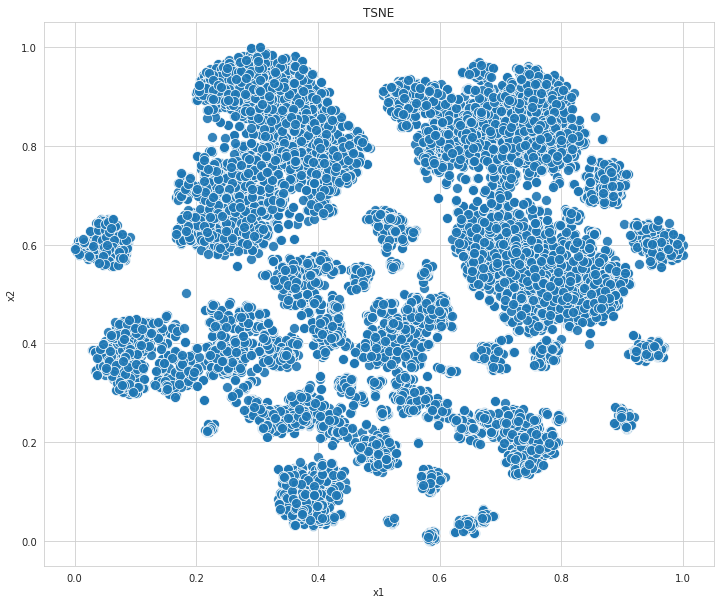
\includegraphics[width=\linewidth]{example1-clustering-products-fashion-tex/output_57_1}
  \caption{Preliminary visualisation of \textit{objective data} in 2-D projection with T-SNE dimensionality reduciton.}
  \label{fig:tsne}
\end{figure}
If data have an underlying structure, points representing observations will cluster, which would be observed on the chart.
As T-SNE on massive data could be resource intensive, the default is to run this process on random subsample and cache results.
Additionally, users can apply textual labels to the T-SNE chart, plotted on a subsample of data, to avoid cluttering the chart. % , prepared in {Data preparation}
Labels could represent the most important pieces of \textit{metadata}, such as the label, the observation id, and summary of description.
The next clue is derived from the silhouette score on a plot in the Figure~\ref{fig:silhouette}.
\begin{figure}[h!]
  \centering
  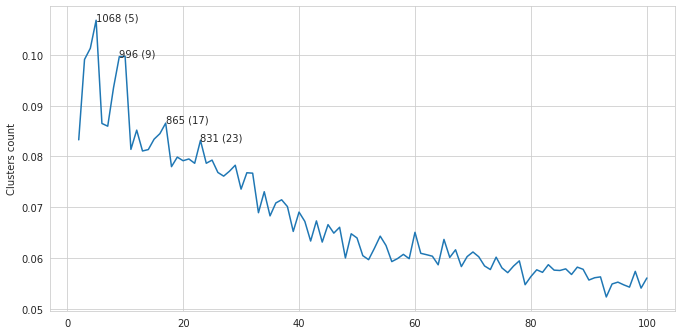
\includegraphics[width=\linewidth]{silhouette-100}
  \caption{Silhouette score with cluster counts and values.}
  \label{fig:silhouette}
\end{figure}
The range of the number of clusters to be tested is provided in accordance with the previous clue.
To speed-up computations, this plot could be obtained on a random subset, and results are cached for further reference.
For now, the user interprets the plot on her/his own.
Finally, clustering with k-means is performed on all observations.
Visualization with T-SNE is presented, this time with clusters colored in different colors, which is depicted in Figure~\ref{fig:kmeans}.
\begin{figure}[h!]
  \centering
  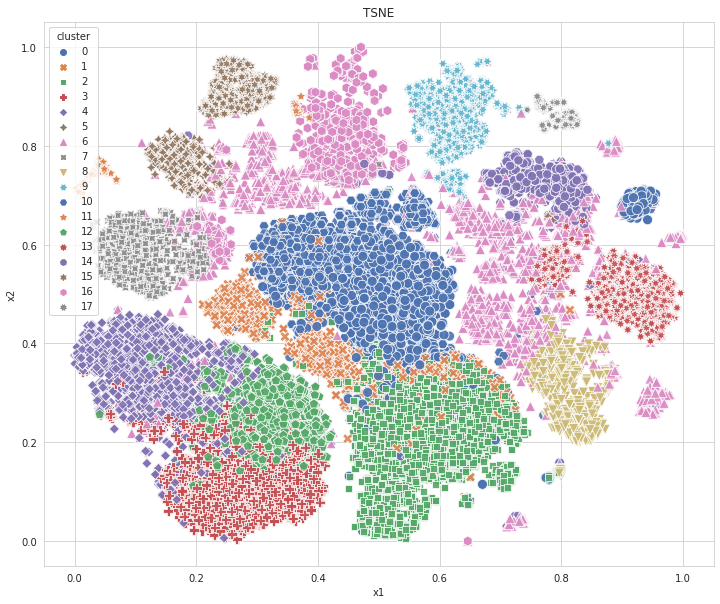
\includegraphics[width=\linewidth]{example1-clustering-products-fashion-tex/output_59_0}
  \caption{Preliminary visualisation of \textit{objective data} in 2-D projection with T-SNE dimensionality reduction. Colors denote clusters discovered with a usage of \textit{objective data}.}
  \label{fig:kmeans}
\end{figure}

\subsection{Interactive explanations}\label{subsec:interactive-explanations}
%- then textual explanations follows straight away
\begin{figure}[h!]
  \centering
  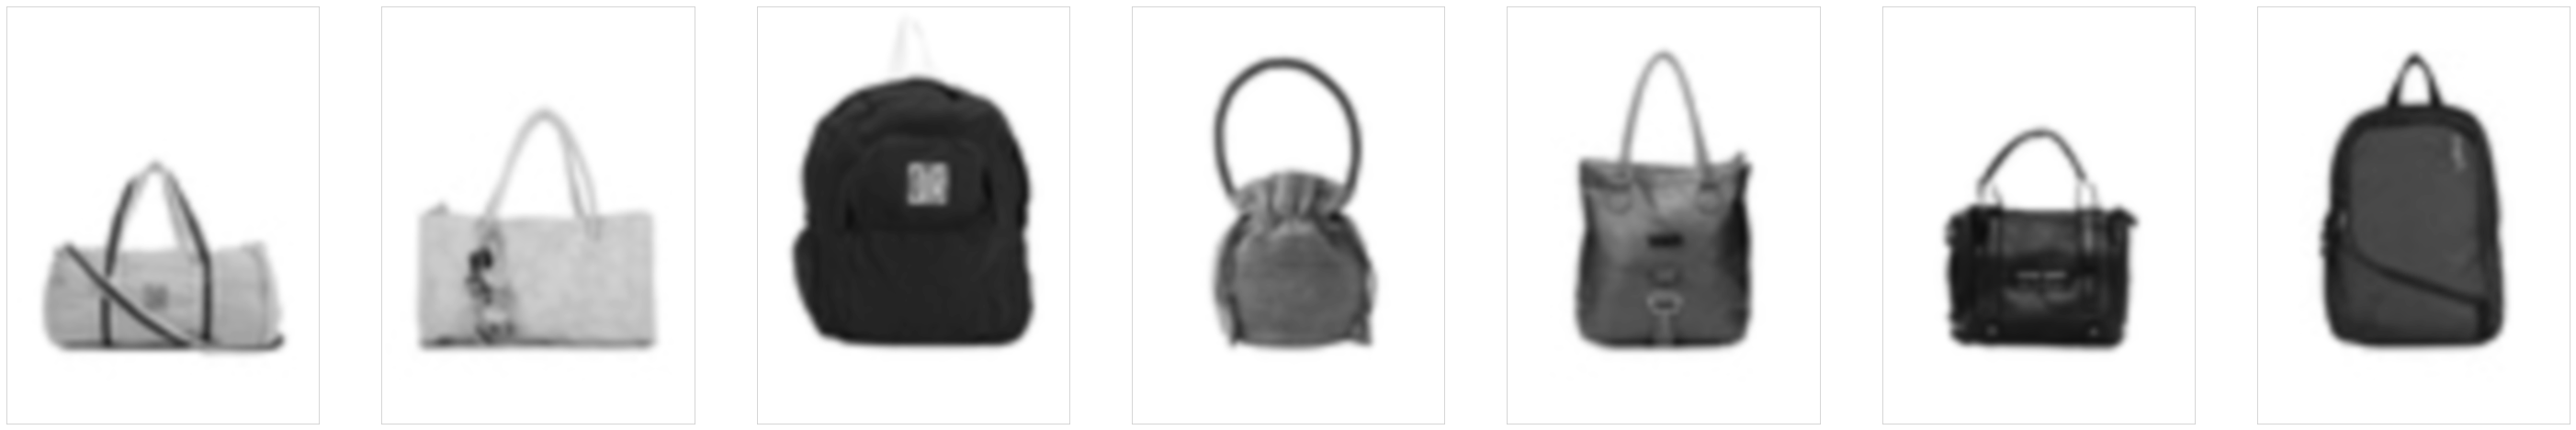
\includegraphics[width=\linewidth]{example1-clustering-products-fashion-tex/output_62_22}
  \caption{Example images of products that were assigned to the same cluster 13 based on the \textit{objective data}.}
  \label{fig:example_products}
\end{figure}

\begin{figure}[h!]
  \centering
  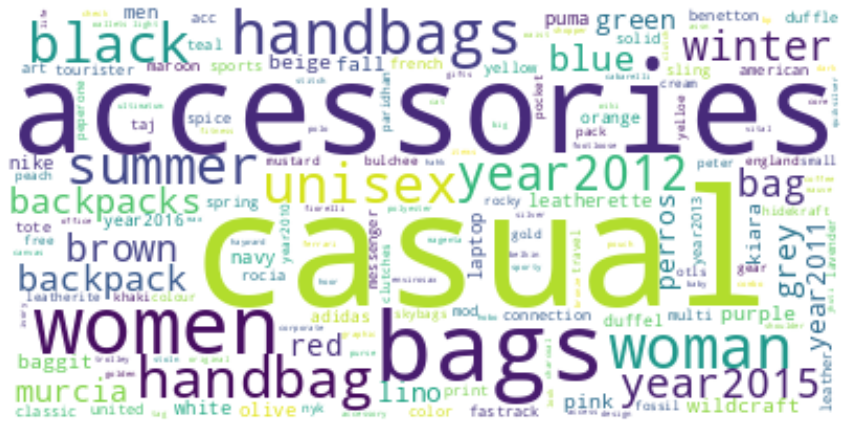
\includegraphics[width=\linewidth]{example1-clustering-products-fashion-tex/output_62_23}
  \caption{Word cloud for a cluster of products presented in Fig.~\ref{fig:example_products} (cluster 13) generated with \textit{metadata}.}
  \label{fig:wordcloud}
\end{figure}

The second step is to explain the clusters so that the person performing the data analysis can assess the result.
We would like to give users the freedom to refine explanations.
Thus, we provide her or him with the possibility to influence explanations by extending stopwords with his own terms.
On the other hand, we initialize the whitelist with keywords like "year2022", defined in "step 0".
Then we use the Tf-Idf vectorizer, taking into account the aforementioned lists.
Vectors are used to train decision tree classifiers.
The size of the list of additional terms is under the control of a user.
She or he can change it and interactively observe the result in a Figure~\ref{fig:decision_tree}, which gives an insight into what terms were relevant for classifier.
Furthermore, for every cluster, example observations, word clouds and LIME explanation for description of random observation are presented.
For instance for the cluster 13 in Figure~\ref{fig:example_products} one can see example products, word clouds that describe clusters in Figure~\ref{fig:wordcloud} and LIME~\cite{lime} explanation for one instance of \textit{metadata} in Figure~\ref{fig:lime}.
In this case one can see that the cluster 13 corresponds to product category "handbags".

\begin{figure*}[h!]
  \centering
  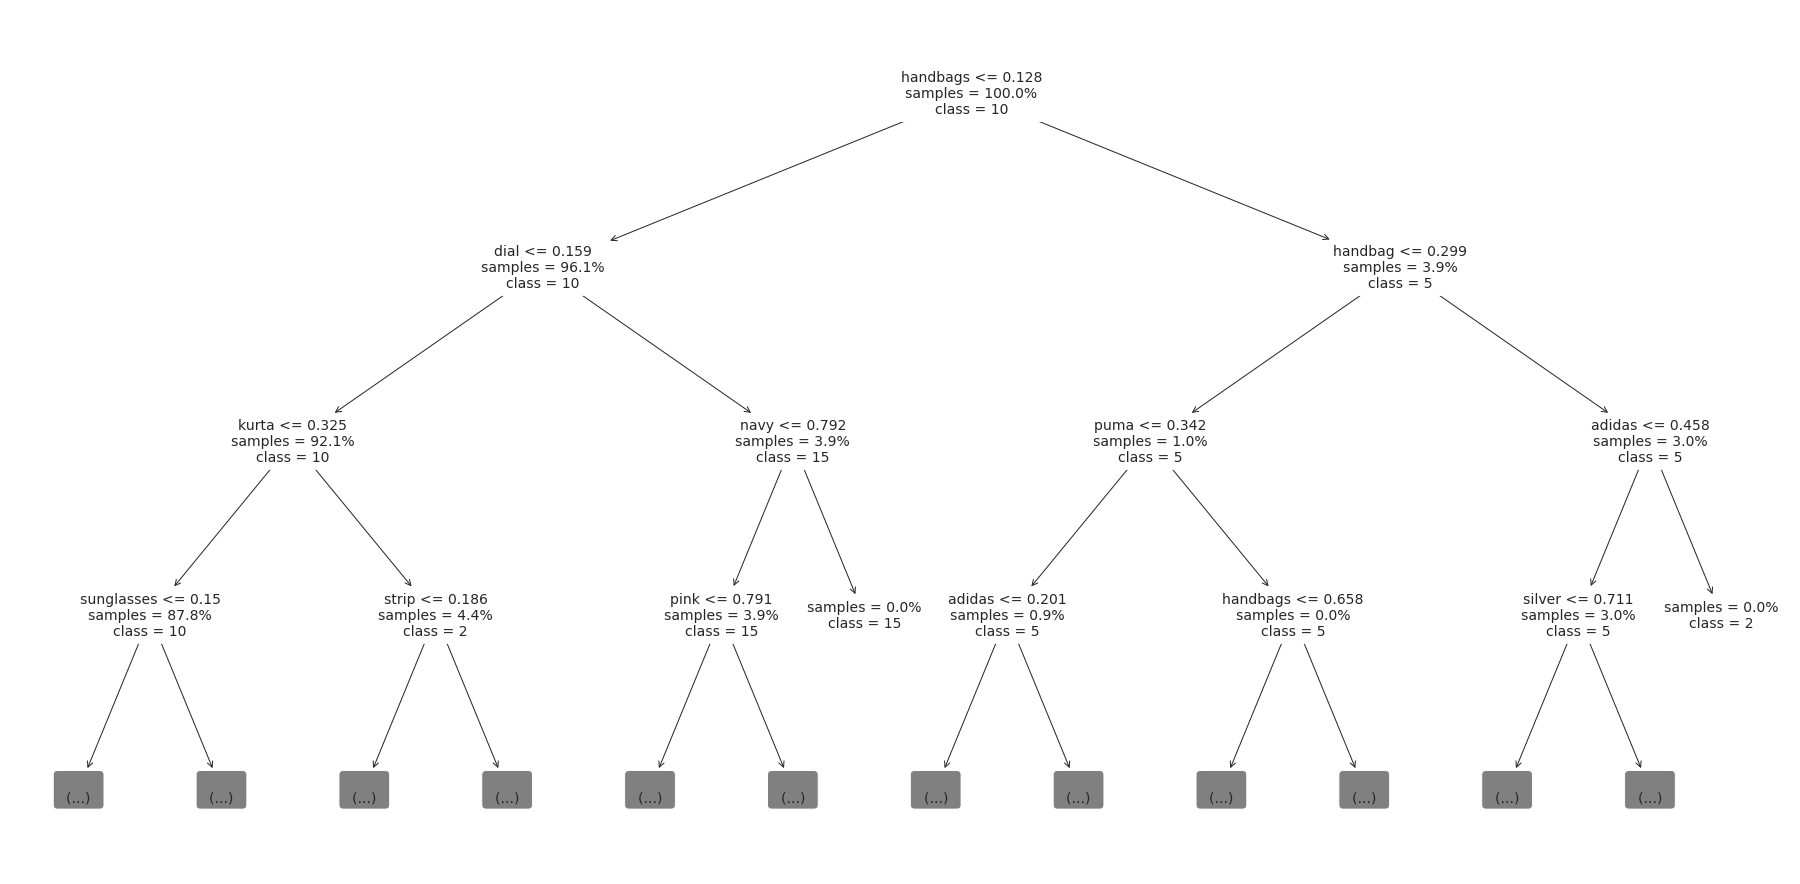
\includegraphics[width=0.8\textwidth]{tree-improved}
  \caption{Decision tree classifier which explains how clusters differ in terms of \textit{metadata}, here pruned to level 4.}
  \label{fig:decision_tree}
\end{figure*}

\begin{figure*}[h!]
  \centering
  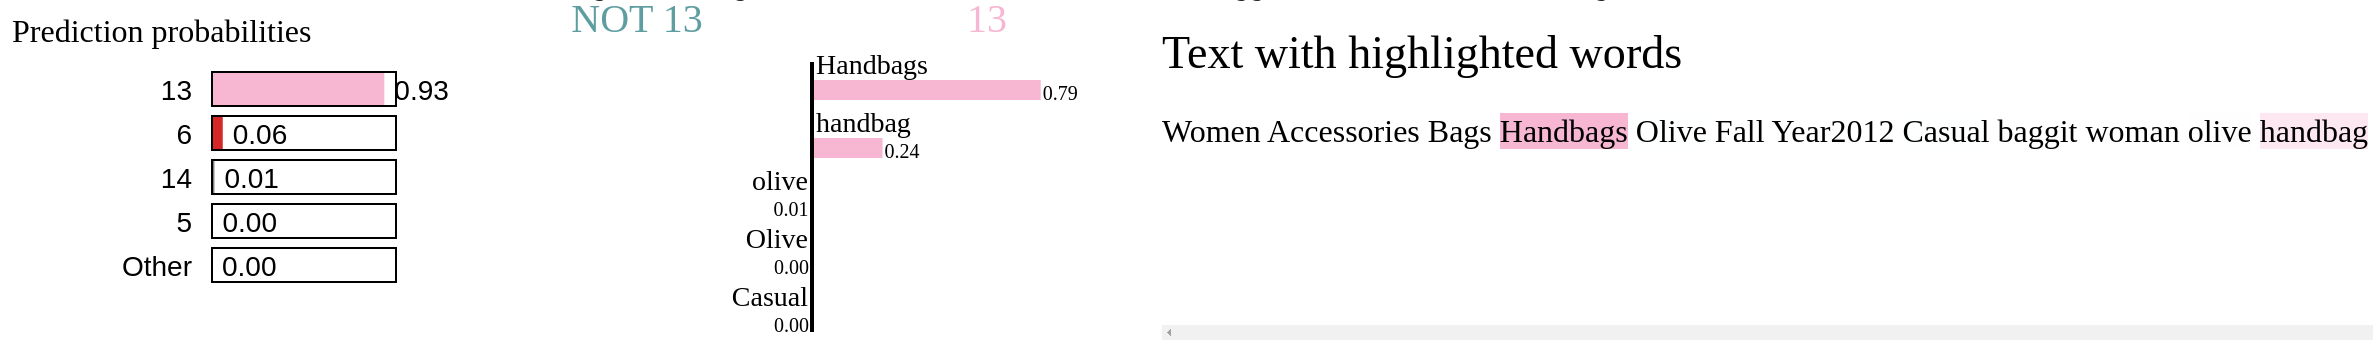
\includegraphics[width=0.8\textwidth]{example1-clustering-products-fashion-tex/LIME_13_handbags-Selection_265}
  \caption{LIME explanation for a random observation drawn from the cluster 13.}
  \label{fig:lime}
\end{figure*}

The last stage is a plot of the word cloud of each cluster, using the same Tf-Idf vectorizer.
Plots are accompanied by examples of observations.% if data scientists should define visualization function and pass into Pipeline class API\@.
In addition, a user is presented an explanation generated with LIME for a random instance from a given class.
The whole process is iterative, and the expert decides on its convergence.

%\section{Real case scenario}
%So far we tested our approach on 2 cases.
%We provide user with Pipeline class, which works in Python environment, like Jupyter notebooks.
%%, which API consist of methods:
%%About the paper citation clustering  and what are plans for extending that part.
%
%Textual data was processed as follows:


\section{Summary}
\label{sec:summary}
%We believe that the XAI methods are most useful when they support human work.
%The main purpose of this paper is to show that XAI can be put into practice when it is based on 2 foundations.
%The first is the need for a dialogue between the machine learning system and its user, taking into account the needs and predispositions of the latter.
In this work, we presented the method that allows for explaining clusters with concepts that could be more human-readable than the data which was used as an input to clustering algorithm.
We based our method on the observation that different types of data are suitable in different degrees to clustering and explaining tasks.
We demonstrated the feasibility of our approach on the e-commerce example, where images were treated as input for clustering and textual descriptions of images as basis for cluster descriptions.

In its current version, the system shows some adaptability to the needs of a human expert.
\textit{Metadata}-based explanations can be refined in two ways.
The user can influence the number of tokens used in the explanation or can directly influence the list of tokens by adding words to the whitelist or blacklist.
After each such change, the expert can see how it affects the classifier used as an explainer, both globally and at the level of random observations for a cluster.
One can modify the scope of the \textit{metadata} and the way individual observations are presented.
If the results, despite the changes, are not satisfactory, it may imply the need to go back to choosing the number of clusters.

%Our approach is obviously not new, but it is worth emphasizing if one wants to create useful solutions for machine learning practitioners.
%We have developed a method that relates to the cluster analysis method, as this technique is widely used with a broad spectrum of applications in science, industry, business, and marketing.
%Furthermore, it is easy to show that it is actually a technical extension of the natural process of describing reality.
%It is also clearly an iterative process, so it is a form of a dialogue between humans and algorithms, and understanding is even more important than, for example, in regression techniques.

%- deep learning - how to use \textit{metadata} in DL ?
%- NLG for explanations
In future work we would like to improve our method with several extensions.
We will focus on automatically proposing number of clusters based on both embedding features with methods similar to T-SNE and metrics like silhouette score.
We want to test clustering techniques other than k-means.
For instance, hierarchical clustering could be more suitable in e-commerce, where taxonomies of products are multilayer.
Word clouds could be replaced with topic analysis with Latent Dirichlet Allocation or techniques derived from Natural Language Generation.
Another interesting direction is to construct explanations with other modalities, like visual, by something more sophisticated than presenting example images.
It could be done for instance with image captioning.


%We are already working on applications of the tool
%- e-commerce: customer segmentation, SEO
%-

\begin{acknowledgments}
  This paper is funded from the XPM (Explainable Predictive Maintenance) project funded by the National Science Center, Poland under CHIST-ERA programme Grant Agreement No. 857925 \\ (NCN UMO-2020/02/Y/ST6/00070).

  The work of Szymon Bobek has been additionally supported by a HuLCKA grant from the Priority Research Area (Digiworld) under the Strategic Programme Excellence Initiative at the Jagiellonian University (U1U/P06/NO/02.16).

  The work of Samaneh Jamshidi was supported by CHIST-ERA grant CHIST-ERA-19-XAI-012 funded by Swedish Research Council.

  The work of Maciej Mozolewski has been additionally supported by Edrone Sp. z o.o.\footnote{See: \url{https://edrone.me/en/}}, which provided computer resources for machine learning.
\end{acknowledgments}

%%
%% Define the bibliography file to be used
\bibliography{sample-ceur}
\end{document}

%%
%% End of file
